
\documentclass[10pt]{article}
\usepackage[margin=1in]{geometry}
\usepackage{amsmath, amssymb, setspace, graphicx, caption, listings, enumitem, subfigure, float}



\begin{document}

\title{ECE 4750 Lab 5: Multicore Processor}
\author{Avinash Navada (abn44) \& Akshay Dongaonkar (akd54) 
		\& Vivek Gaddam (vrg22)}
\maketitle


\section{Introduction}

Modern computing applications are becoming increasingly calculation-intensive and Moore's Law is yielding diminishing returns, highlighting the need for alternative ways to improve overall processor performance. Parallelizing independent work over multiple execution cores is one way to increase throughput and take advantage of thread-level parallelism. However, such systems come with added complexity and their performance relies on design choices such as the particular
cache and on-chip interconnect network schemes used. \par

In this lab, we implement and analyze the benefits of using a quad-core system with a banked data cache and private instruction caches per core over a single-core system with single data and instruction caches by comparing their performance on a set of single and multithreaded microbenchmarks. In doing so, we can gain insight into the specific area, energy, and performance tradeoffs between these setups and draw conclusions on when one system might be more appropriate than the other. \par

The baseline design is the single-core setup, and the alternative design is the quad-core setup. In completing both designs, we ultimately found that in terms of total number of cycles per program, multithreaded microbenchmarks run on the alternative design performed approximately 2 times better than did single-threaded versions of the same benchmarks run on the baseline. Based on these simulation results, we would choose the alternative multicore implementation over the baseline implementation if performance is of the highest priority. However, the multicore processor requires much more logic and energy (assuming the same clock frequency) compared to the baseline and so if cost, complexity, area, and energy are also important considerations, the design of choice may be either the single-core or the multicore processor. 



\section{Project Management}

% 
For this lab, all testing was provided. Therefore, we split the remainder of the work amongst ourselves as follows:
-Avinash wrote the RTL code for the baseline and alternative designs composing the processor cores, caches, and network.
-Akshay wrote the version of the quicksort algorithm to be run on the baseline design and parallelized it for testing on the alternative design.
-Vivek helped optimize the quicksort C algorithm and was the lead in writing the lab report. \par

Our expected and actual work patterns are shown in Figure~\ref{fig:gantt}.


\section{Baseline Design}

The baseline design for this lab report is a single-core system consisting of a fully bypassed pipelined PARCv2 
processor interfaced with a two-way set-associative instruction cache and a two-way set-associative data cache. 
The processor communicates with an external source and sink for testing purposes. All interfaces between these
components are val-ready to allow for composing a variety of different implementations. \par

Due to an existing bug in our pipelined processor from Lab 2, we decided to use the provided processor core, 
cache, and network units in composing our baseline design. Our design is in accordance with the setup in 
Figure~\ref{fig:bline}. This overall setup is responsible for fetching assembly instructions from a provided
instruction memory and accessing a provided data memory when needed in order to execute programs.

Because our baseline design is composed entirely of components that were designed in previous labs that were 
tested individually, specifically the caches and processor core, it is a good example of a modular design. 

This design can be viewed as the minimum hardware one expects to have when running full C programs, and is therefore
an appropriate baseline for comparison to more complicated designs, such as the quad-core processor that serves as
our alternative design. Any real system should include caches for instruction and data memories to reduce the average memory
access latency (AMAL), so it makes sense for our baseline implementation to use them as well. 

We also implemented the quicksort sorting algorithm in C for use on one core. This was used as a microbenchmark in our lab. This was a straightforward quicksort algorithm implementation (we referred to http://algs4.cs.princeton.edu/23quicksort/ for clarifications on quicksort). A slight optimization that we provided in our lab was to amortize copying the contents of the source array over to the destination array as the first quicksort iteration was performed, which may result in the reduction of a small number of assembly instructions, depending on the compiler.

% Diagram of base datapath or block diagram


\section{Alternative Design}

In our alternative design, our processor consists of four cores each identical to the one in the baseline design and compose them with four two-way set-associative instruction caches and four two-way set-associative data caches. Of course, this composition of multiple processor cores and caches must still behave externally as a single execution unit that takes instructions from a single instruction memory and uses a single data memory, just as the baseline design does. Therefore, we must coordinate the separate entities with networks. We have request/response ring networks between the caches and their respective memory interfaces in addition to ring networks between the caches and the processor cores. The request/response networks arbitrate multiple requesters over the single memory port and route memory response data to the correct requester. We also use a separate interconnect network between the datacaches and processor cores to support shared data caching. See Figure~\ref{fig:alt} for the datapath of our alternative design.

One important feature of the alternative design is that it uses a single banked data cache. In a typical multithreaded application, threads will provide parallelism by performing significant amounts of calculation on some sort of common state. Two observations come from this: first, that the threads will likely access and modify large numbers of data addresses (e.g. while streaming through a large array), and second, that the data is shared amongst the threads, regardless of whether or not the threads are performing the same type of work on that data. A banked data cache is a response to both of these observations. Given some fixed technology constraints such as a restriction on area devoted to caches, we would like to use the data caches as effectively as possible. Therefore, we would like to share the allowed cache space amongst all threads (to make the cache as big as possible), allowing any particular data address to live in only one place in the shared cache at a time. We do not however bank the instruction caches here; we decide not to always pay the overhead of having a network arbitrate a single banked instruction cache over multiple execution cores when in fact having a banked instruction cache does not necessarily make sense for multithreaded applications.

In some ways, the quicksort application we implement in this lab does not fit this above profile of a multithreaded program. Each thread executes identical instructions (with respect to IPC) but may in fact modify completely disjoint parts of the input array. Nevertheless, we may not typically have such fine parallelization. Furthermore, notice that a single thread is likely to use many different data addresses much quicker than it does distinct instruction PCs in a given timeslice in a typical scenario like looping over a large array. Therefore, even if there are duplicate entries across the private instruction caches, they are likely to live there for many cycles. As always, we try to optimize some scenarios over others while still providing functionality over a wide array of uses.

We would like to see how close our alternative design can come to actually realizing the ideal performance benefit of having four cores with the knowledge that the additional cores, caches, and network infrastructure required come with some energy and performance cost.


\section{Testing Strategy}

As mentioned earlier, the testing suite for this lab was provided to us and consisted of single-threaded source/sink based tests as well as single and multi-threaded self-checking assembly tests. The source/sink tests comprehensively test all PARC v2 instructions compiled for the PARC ISA. The self-checking tests dynamically test each instruction and check for correct simulation output on their own based off of status signals from the DUT. For the baseline design, we first connected the different components and then ran the source/sink tests. When the source/sink tests passed, we tried running the self-checking tests on the processor and ensured that they worked before proceeding to run the benchmarks on the processor. These benchmarks ensured that our implementation worked for programs with many instructions and/or greater complexity. A similar testing strategy was adopted for the alternative design (although there were no source/sink based tests specially written for testing multithreading). Since the alternative RTL was a lot more complex than the baseline given the network, port picking, and varying bitwidths, VCD dumps had to be carried out in addition to having to run the source/sink and self-checking tests many more times than we had to for the baseline. One issue we noticed was that the multithreaded quicksort code compiled and ran natively as well as on the alternative implementation when tested separately but failed on the simulator. Ultimately, both our baseline and alternative designs passed all tests and benchmarks. 



\section{Evaluation}

By running the various single-threaded and multithreaded microbenchmarks on the single-core and multicore systems, we can get an idea for how their performance compares. \par

As shown in Table~\ref{tab:eval}, the alternative design generally provides an approximately 2x speedup on all the applications over the baseline design. Note that we assume that both designs have the same cycle time, so that we can compare the designs by comparing their performances in cycles. This appears to be a reasonable assumption: we do not seem to have introduced any long pathways between clocked units going from the baseline design to the alternative design. It is important to note that in real-world processors, the processor may be downclocked to reduce power consumption and to stay within TDP constraints, especially given that mobile devices that require low processor power consumption are an increasingly high priority for chip manufacturers. \par

For the binary search and masked filter applications, we get almost exactly a 2x speedup in performance when going from baseline design to alternative, with binary search going from 12205 cycles to 6187 cycles and masked filter going from 25596 cycles to 12827 cycles. These operations, like the quicksort, are well-suited to multithreading and therefore we do expect large performance gains. However, as mentioned in the lab handout, ``a fully parallelized application running on N processors would speedup by 4x'', which we do not see here. We can expect this trend to continue with adding more parallel processing units resulting in additional speedup in executing instructions given comparatively efficient parallelization algorithms and sufficient independent work that can be parallelized across threads/processes. \par

Note that the CPI in Table~\ref{tab:eval} is total cycles per program over instructions \textit{per core}. So, while CPI appears to balloon after adding more cores, we still get a significant speedup overall by parallelizing. It is important to note here that CPI goes into the first-order processor performance equation, not total cycles per program. So that would mean that the alternative implementation performs more poorly compared to the baseline implementation according to the first-order equation. However, the first-order equation does not apply to multicore processors like the one implemented here and so total number of cycles per program is a more appropriate measure of comparison between the two designs, especially considering that the instructions per program and time/cycles variables are the same for both. \par

Clearly, the alternative design, with its multiple cores and cache units, takes up more area than the baseline design. Given that having multiple cores also necessitates the use of networks, we would expect the alternative design to take up more than 4x the amount of area taken up by the baseline design.

The alternative design also appears to use more power (energy per time) than the baseline. It has four execution cores and presumably many more cache requests per cycle, not to mention the extra energy expended in traversing the various interconnect networks and in the additional computations required in the multicore system's control unit to synchronize the threads across cores. These extra costs could potentially outweigh any potential gains the multicore system might have over the single-core configuration on a typical multithreaded program, gains such as requiring fewer data memory accesses due to having a larger banked data cache and requiring less cache evictions. It would all depend on the relative importance of the criteria of performance, cost, energy, and area to the designer (in turn usually dictated by application requirements and other considerations). Collectively, we expect a large (>4x) power consumption increase from the baseline to alternative design assuming a constant clock frequency. Given that we do not get a matching performance increase in terms of number of cycles from baseline to alternative, we may conclude that the alternative design also eats up more energy per program than does the baseline.

Overall, we pay extra area, energy and power costs to get greater performance in the quad-core system over the standard single-core system.



\newpage
\section {Tables and Diagrams}

% Figure: Gantt Chart
% \begin{figure}[H]
% 	\centering
% 	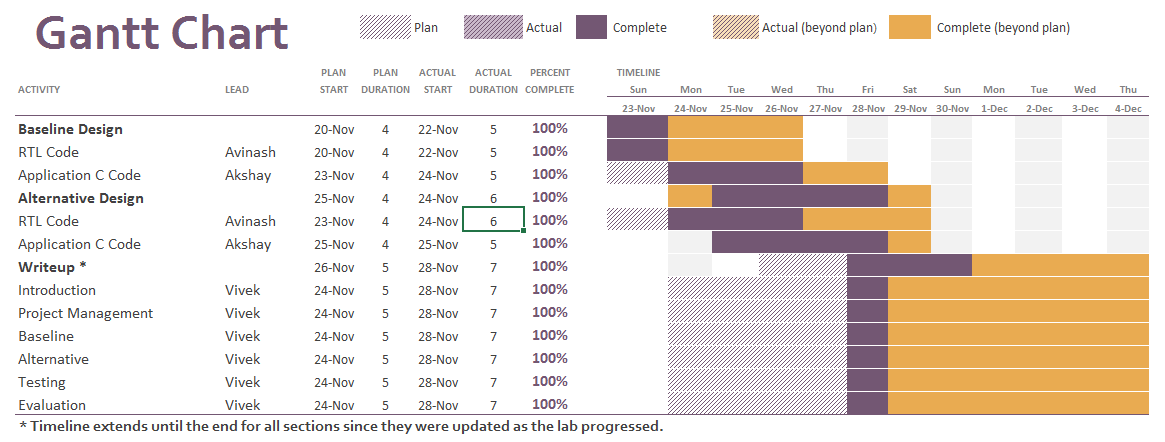
\includegraphics[scale=0.4, angle=90]{gantt}
% 	\caption{Gantt Chart.}
% 	\label{fig:gantt}
% \end{figure}

% Figure: Baseline Design
\begin{figure}[H]
	\centering
	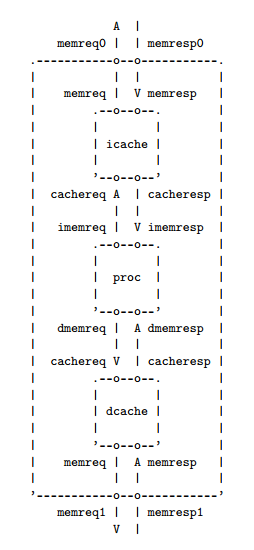
\includegraphics{bline_diag}
	\caption{Baseline Design - Single-Core system}
	\label{fig:bline}
\end{figure}

% Figure: Alt Design
\begin{figure}[H]
	\centering
	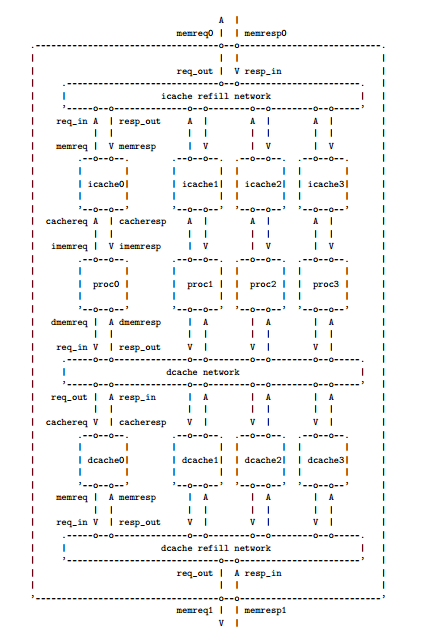
\includegraphics{alt_diag}
	\caption{Alternative Design - Multi-Core system}
	\label{fig:alt}
\end{figure}

% EVALUATION: Summary Table
\begin{table}[H]
\centering
	\begin{tabular} {|l | r | r | r |}
	\hline
	\textbf{Design}    & \textbf{Cycles} & \textbf{Instructions} & \textbf{CPI} \\
	\hline
	Baseline - vvadd       		&  2294  &  502   &  4.97   \\
	Baseline - cmplx-mult  		&  9080  &  1972  &  4.6  	\\
	Baseline - bin-search       &  12205 &  2658  &  4.59   \\
	Baseline - masked-filter    &  25596 &  5742  &  4.46   \\
	Baseline - quicksort        &  ----  &  --    &      	\\
	\hline
	Alternative - vvadd    		&  1812  &  233   &  7.78   \\
	Alternative - cmplx-mult    &  5525  &  641   &  8.62   \\
	Alternative - bin-search    &  6187  &  926   &  6.68   \\
	Alternative - masked-filter &  1287  &  1992  &  6.44   \\
	Alternative - quicksort    	&  ----  &  --    &         \\
	\hline                    
	\end{tabular}
	\caption{Baseline v. Alternative Design Performance}
	\label{tab:eval}
\end{table}

% END
\end{document}